\documentclass{article}
\usepackage[utf8]{inputenc}
\usepackage[english,ngerman]{babel}
%% ========================================================================
%%%% MISC usepackages
%% ========================================================================

%% Chemistry
\usepackage{chemfig,chemmacros}
\chemsetup{modules = all}
\chemsetup[redox]{explicit-sign = true}
\chemsetup[phases]{pos=sub}
%\chemsetup[reactions]{before-tag = {R}, tag-open = [, tag-close = ]}
  
%% Maths
\usepackage{amsmath,amssymb,amsthm,textcomp}

%% Physics
\usepackage{siunitx}

%% Graphics
\usepackage{graphicx}
\usepackage{tikz}
\usepackage{rotating}
%\usepackage{subfig}

%% Tables and Lists
\usepackage{enumerate}
\usepackage{multicol}
\usepackage{geometry}
\usepackage{tabu}
\usepackage{listings}
\usepackage{tabularx}

%% Structures and Style
\usepackage{caption}
\usepackage{subcaption}
\usepackage{booktabs}
\usepackage{colortbl}

\usepackage{xcolor}
\usepackage{xfrac}
\usepackage[export]{adjustbox}[2011/08/13]

\usepackage{booktabs}
\usepackage{float}

\usepackage{fancyhdr}

%% Citing and Settings
\usepackage[backend=biber,
style=numeric,
backref=true, 
natbib=true, %% offering natbib-compatible commands
hyperref=true, %% using hyperref-package references
sorting= none,
doi=true,
maxcitenames=10,
maxbibnames=100,
citestyle=numeric
]{biblatex}

\addbibresource{references.bib}

\usepackage[toc,automake]{glossaries}
\include{abbrevations}
\makeglossaries

\usepackage[colorlinks=true,linkcolor=blue]{hyperref}

%% Figure settings
\renewcommand{\figurename}{Abbildung}
\renewcommand{\tablename}{Tabelle}
\renewcommand{\listfigurename}{Abbildungsverzeichnis}
\renewcommand{\listtablename}{Tabellenverzeichnis}

%% ========================================================================
%%%% Document Information
%% ========================================================================

%% Title
\title{Bestimmung der Gleichgewichtskonstante für ein heterogenes Gleichgewicht \cite{Versuchsvorschrift}} % Title
\author{Autor: Florian \textsc{Kluibenschedl}} % Author name
\date{Bericht verfasst am: \today} % Date for the report

% Page style - headers
\pagestyle{fancy}
\fancyhf{}
\rhead{PR Allgemeine Chemie A - SS2019}
\lhead{Institut für Allgemeine Chemie - Universität Innsbruck}
\rfoot{Experiment 6 - Seite \thepage}


\begin{document}
  \renewtagform{reaction}[Rgl. ]{}{}
  
  \maketitle % Insert the title, author and date
  
  \begin{center}
    \begin{tabular}{r p{4cm}}
      Versuchsdurchführung am: & 12. März 2019\\ % Date the experiment was performed
      Gruppe, Matrikelnummer: & 3, 11805747 \\
      Lehrveranstaltung: & PR Allgemeine Chemie A \\
      Institut: & Allgemeine, Anorganische und Theoretische Chemie \\
      Assistent: & Kriesche Bernhard % Instructor/supervisor
    \end{tabular}
  \end{center}


  \begin{abstract}
    Gleichgewichtskonstanten spielen eine bedeutende Rolle in der Chemie. Insofern ist es un-
umgänglich, Methoden ihrer Bestimmung zu kennen.

    In diesem Experiment wurde über Titration das Löslichkeitsprodukt von \ch{PbI2\sld} bestimmt. Dazu wurde eine \SI[mode=text]{0.50}{M} \ch{Pb(NO3)2} Lösung mit einer \SI[mode=text]{0.020}{M} \ch{KI} Lösung titriert. Endpunkt der Titration war eine gelbliche Trübung der Lösung. Das Löslichkeitsprodukt wurde durch Extrapolation des gemessenen, von der Gesamtkonzentration unabhängigen Löslichkeitsprodukt bestimmt. Dazu wurde Mathematica verwendet. Die auf diese Weise erhaltenen Werte sind: $K_{L}=\num{3.66d-9}$, $L_{M} = $\SI[mode=text, separate-uncertainty]{9.70d-4}{\mole\per\liter} $\equiv$ \SI[mode=text, separate-uncertainty]{0.45}{\gram\per\liter}. Ein Vergleich mit dem Literaturwert ($K_{L}=\num{9.8d-9}$ bei \SI[mode=text]{25}{\degreeCelsius} \cite[S. 8-819]{solubilityConstants}) zeigt, dass die Bestimmung recht genau war.  
    
     
  \end{abstract}
  
  \pagebreak
  
  \section{Theoretische Grundlagen}
  
    \subsection{Motivation} \label{sec:Motivation}
    
      Salze besitzen in Wasser unterschiedliche Löslichkeiten. Kochsalz \ch{NaCl} löst sich beispielsweise sehr gut. Beim gelben \ch{PbI2} handelt es sich um ein schwerlösliches Salz. Die entsprechende Lösereaktion wird in \ref{rec:LosungPblei} beschrieben. 
           
      \begin{reaction}
        PbI2\sld{} <<=> Pb\pch[2]\aq{} +  2 * I\mch\aq{} \label{rec:LosungPblei}
      \end{reaction}
      
      Werden nun zu einer Lösung von \ch{Pb\pch[2]\aq} Ionen \ch{I\mch\aq} Ionen hinzugegeben, fällt \ch{PbI2\sld} aus, wenn das Löslichkeitsprodukt knapp überschritten wird. Dieser Punkt ist erkennbar durch den charakteristischen, gelben Niederschlag von \ch{PbI2\sld}. Es liegt also eine annähernd gesättigte Lösung vor und man kann annehmen, dass das Ionenprodukt von \ch{Pb\pch[2]\aq} und \ch{I\mch\aq} dem Löslichkeitsprodukt entspricht. Ist die Menge an beteiligtem \ch{Pb\pch[2]\aq} und \ch{I\mch\aq} bekannt, kann somit über das Ionenprodukt das Löslichkeitsprodukt berechnet werden.
      
      Da Blei unter anderem giftig ist, ist eine exakte Kenntnis der Bleikonzentration vonnöten, um z. B. zu überprüfen, ob bestimmte Grenzwerte eingehalten werden. Die Konzentration von \ch{Pb\pch[2]\aq} Ionen kann bei bekanntem Löslichkeitsprodukt berechnet werden. \\
      
      Anmerkung zur Angabe von Konstanten im Protokoll: um Probleme mit mathematischen Funktionen wie etwa dem Logarithmus bzw. der Exponentialfunktion zu vermeiden, werden alle Gleichgewichtskonstanten dimensionslos angegeben. Dazu werden alle Spezies im jeweiligen Massenwirkungsgesetz durch die Standardkonzentration ($c_{Standard} = 1 M$) dividiert.
    
    \subsection{Ziel des Experiments}
    
      Auf Basis der obigen Überlegungen ist das Ziel, über Titration eine möglichst exakte Bestimmung des Löslichkeitsproduktes von \ch{PbI2\sld} durchzuführen.
    
    \pagebreak
    
  \section{Experimenteller Teil}
  
    \subsection{Verwendete Materialien}
              
      \begin{table}[H]
        \centering
        \caption[Materialienliste, Quelle: Autor]{Auflistung der verwendeten Geräte und Chemikalien}
        \label{tab:Materialien}
        
        \begin{tabular}{@{}ll|ll@{}}
          \toprule
            Geräte & Hersteller & Chemikalie & Hersteller \\ \midrule
            \SI[mode=text]{600}{\milli\liter} Becherglas & BRAND & \SI[mode=text]{0.50}{M} \ch{Pb(NO3)2} Lösung & Vorrat \\
            \SI[mode=text,separate-uncertainty=true]{25.000(75)}{\milli\liter} Bürette & BRAND & \SI[mode=text]{0.020}{M} \ch{KI} Lösung & Vorrat \\
            \SI[mode=text,separate-uncertainty]{25.000(45)}{\milli\liter} Vollpipette & BRAND & deionisiertes \ch{H2O} & Labor \\
            \SI[mode=text,separate-uncertainty]{100}{\milli\liter} Erlenmeyerkolben & DURAN &  &  \\
            \SI[mode=text,separate-uncertainty]{100}{\milli\liter} Becherglas & DURAN &  &  \\
            digitales Thermometer & TFA Digital &  &  \\
            Stativ mit Klammern &  &  &  \\
            Magnetrührer & CAT M 6.1 &  &  \\
            Rührfisch &  &  &  \\ \bottomrule
        \end{tabular}
      \end{table}
    
    \subsection{Versuchsdurchführung}  \label{sec:Versuch}
    
      Zunächst wurden \SI[mode=text]{25}{\milli\liter} einer \SI[mode=text]{0.50}{M} \ch{Pb(NO3)3} Lösung in einen \SI[mode=text]{100}{\milli\liter} Erlenmeyerkolben pipettiert und mit einer \SI[mode=text]{0.020}{M} \ch{KI} Lösung bis zum Endpunkt titriert. Dabei wurde die Lösung konstant mit einem Rührfisch und Magnetrührer bei ca. \SI[mode=text]{70}{rpm} gerührt. Am Endpunkt war eine gelbliche Trübung der Lösung durch \ch{PbI2\sld} beobachtbar. Das bis zu diesem Punkt benötigte Volumen wurde notiert. Da die gelbe Trübung nicht eindeutig ist, wurden weitere Tropfen \ch{KI} Lösung hinzugegeben und beobachtet, ob die gelbliche Trübung intensiver wurde. War dies der Fall, wurde der notierte Wert genommen.
      
      Die nächsten Titrationen erfolgten bei unterschiedlichen Konzentrationen der \ch{Pb(NO3)3} Lösung. Dazu wurde eine Verdünnungsreihe erstellt. Mit einer Vollpipette wurden \SI[mode=text]{25}{\milli\liter} der \SI[mode=text]{0.50}{M} \ch{Pb(NO3)3} Lösung mit \SI[mode=text]{25}{\milli\liter} deionisiertem Wasser verdünnt. Von der resultierenden \SI[mode=text]{0.25}{M} \ch{Pb(NO3)3} Lösung wurden \SI[mode=text]{25}{\milli\liter} mit der \SI[mode=text]{0.020}{M} \ch{KI} Lösung wie oben beschrieben titriert. Der verbleibende Rest der verdünnten Lösung (\SI[mode=text]{25}{\milli\liter}) wurde mithilfe einer Vollpipette mit deionisiertem Wasser auf \SI[mode=text]{50}{\milli\liter} aufgefüllt. Die resultierende \SI[mode=text]{0.125}{M} \ch{Pb(NO3)3} Lösung wurde wie oben beschrieben titriert und verdünnt. Diese Prozedur wurde wiederholt und man erhielt eine \SI[mode=text]{0.063}{M}, \SI[mode=text]{0.031}{M} und \SI[mode=text]{0.016}{M} \ch{Pb(NO3)3} Lösung. Der Verbrauch an \ch{KI} Lösung sowie die Temperatur am Endpunkt der Titration\footnote{es wurde darauf geachtet, starke Temperaturunterschiede zu vermeiden, da die Löslichkeit stark temperaturabhängig ist und die Ergebnisse sonst nicht vergleichbar wären} wurden jeweils notiert. Die gesättigten \ch{PbI2} Lösungen und andere Bleiabfälle wurden im Schwermetall-Abfall entsorgt.
    
    \pagebreak
    
    \subsection{Auswertung} \label{sec:Auswertung}
      
      Die Konzentration von \ch{Pb\pch[2]\aq} und \ch{I\mch\aq} kann mit dem von der Gesamtkonzentration abhängigen Löslichkeitsprodukt $K_{L,c}$ berechnet werden - siehe \eqref{eq:Klc}. Dabei wird angenommen, dass die Aktivität des Feststoffes \ch{PbI2\sld} gleich eins ist. 
      
      \begin{equation}
        K_{L,c} = \frac{a_{\ch{Pb\pch[2]\aq}} * a_{\ch{I\mch\aq}}^2}{a_{\ch{PbI2\sld}}} = a_{\ch{Pb\pch[2]\aq}} * a_{\ch{I\mch\aq}}^2 = f_{\ch{Pb\pch[2]\aq}} [\ch{Pb\pch[2]\aq}] * f_{\ch{I\mch\aq}}^2 [\ch{I\mch\aq}]^2 \label{eq:Klc}
      \end{equation} 
      
      Unter der Annahme, dass die Wechselwirkungen zwischen den Ionen und Molekülen der Lösung vernachlässigt werden können, ergibt sich aus \eqref{eq:Klc} das bekannte Löslichkeitsprodukt $K_{L}$ - siehe \eqref{eq:Kl}. Es gilt also $\lim_{c_{ges.}\to 0} f_{i} = 1 \Leftrightarrow \lim_{c_{ges.}\to 0} K_{L,c} = K_{L}$.
      
      \begin{equation}
        K_{L} = [\ch{Pb\pch[2]\aq}] * [\ch{I\mch\aq}]^2 \label{eq:Kl}
      \end{equation} 
      
      Die symbolische Konzentration von \ch{PbI2} in der Lösung wird durch die Löslichkeit $L_{M}$ ausgedrückt. Sie errechnet sich aus dem Löslichkeitsprodukt - siehe \eqref{eq:solubility}.
      
      \begin{equation}
        L_{M} = [\ch{Pb\pch[2]\aq}] = \frac{1}{2} [\ch{I\mch\aq}] = \sqrt[3]{\frac{K_{L}}{4}} \label{eq:solubility}
      \end{equation} 
      
      Im Folgenden werden weitere Beziehungen angegeben, die für die Berechnung der Werte in Tabelle \ref{tab:Messdaten} benötigt wurden. Die Berechnung von [\ch{Pb(NO3)3}] wird nicht angeführt, da dies bereits in \ref{sec:Versuch} erledigt wurde.
      
      \begin{equation}
        pK_{L,c} = -\log_{10} (K_{L,c})
      \end{equation}
      
      \begin{equation}
        V_{Ende} = V_{\ch{KI}} + V_{\ch{Pb(NO3)3}}
      \end{equation}
      
      \begin{equation}
        [\ch{Pb\pch[2]\aq}]_{eq.} = \frac{[\ch{Pb(NO3)3}] * V_{\ch{Pb(NO3)3}}}{V_{Ende}}
      \end{equation}
      
      \begin{equation}
        [\ch{I\mch\aq}]_{eq.} = \frac{[\ch{KI}] * V_{\ch{KI}}}{V_{Ende}}
      \end{equation}
      
    \pagebreak
      
    \subsection{Messergebnisse und Literaturwerte}
    
      In Tabelle \ref{tab:Messdaten} sind alle Messwerte angeführt, die im Rahmen der Versuchsdurchführung wie in \ref{sec:Versuch} beschrieben, gemessen wurden. Volumina sind in L, Konzentrationen in M angegeben. Die einzelnen aus den Messdaten errechneten Werte wurden gemäß den in \ref{sec:Auswertung} angeführten Beziehungen berechnet.
      
      \begin{table}[H]
        \centering
        \caption[Messdaten und daraus abgeleitete Größen, Quelle: Autor]{Messdaten und daraus abgeleitete Größen}
        \label{tab:Messdaten}
          \begin{tabular}{@{}l|llll|ll|lll@{}}
            \toprule
             Nr. & $V_{\ch{Pb(NO3)3}}$ & [\ch{Pb(NO3)3}] & $V_{\ch{KI}}$ & $V_{Ende}$ & $[\ch{Pb\pch[2]\aq}]_{eq.}$ & $[\ch{I\mch\aq}]_{eq.}$ & $K_{L,c}$ & $pK_{L,c}$ & T in \si{\kelvin} \\ \midrule
             1 & 0.025 & 0.50 & 0.0054 & 0.0304 & 0.41 & 0.0036 & \num{5.19d-6} & 5.285 & 296.3 \\
             2 & 0.025 & 0.25 & 0.0036 & 0.0286 & 0.22 & 0.0025 & \num{1.39d-6} & 5.859 & 296.7 \\
             3 & 0.025 & 0.125 & 0.0024 & 0.0274 & 0.11 & 0.0018 & \num{3.50d-7} & 6.456 & 297.1 \\
             4 & 0.025 & 0.063 & 0.0018 & 0.0268 & 0.058 & 0.0013 & \num{1.05d-7} & 6.978 & 297.1 \\
             5 & 0.025 & 0.031 & 0.0015 & 0.0265 & 0.030 & 0.0011 & \num{3.78d-8} & 7.422 & 296.8 \\
             6 & 0.025 & 0.016 & 0.0013 & 0.0263 & 0.015 & 0.00099 &  \num{1.45d-8} & 7.839 & 296.6 \\ \bottomrule
          \end{tabular}
       \end{table}      
      
  \section{Ergebnisse und Diskussion}
    
    Aus den in Tabelle \ref{tab:Messdaten} angegebenen Daten errechnen sich folgende Werte: $K_{L,c} = $ \num[separate-uncertainty]{1.18 \pm 2.03 e-6} ($s = \num{\pm 2.03d-6},\alpha=0.05,N=6$), $pK_{L,c} = $ \num[separate-uncertainty]{5.33 \pm 2.72} ($s=\num{\pm 2.72},\alpha=0.05,N=6$).\\
    
    Um nun einen Ausdruck für $K_{L}$ zu erhalten, wird eine Extrapolation durchgeführt. Dazu wurden zwei Programme verwendet. 
    
    Im Folgenden werden die Ergebnisse der Extrapolation mit LibreOfficeCalc \cite{LibreOffice} diskutiert. Eine Auftragung der $pK_{L,c}$ Werte von Tabelle \ref{tab:Messdaten} gegen $[\ch{Pb\pch[2]\aq}]_{eq.}$ ergibt Diagramm \ref{fig:Extrapolation}. Das Modell, das diese Punkte statistisch am besten beschreibt, ist ein quadratisches (die Gleichung wird in \ref{fig:Extrapolation} angegeben). Wird dieses Polynom an der Stelle null ausgewertet, erhält man den Wert für $pK_{L}=7.862$ und daraus errechnet sich folgender Wert für das gesuchte Löslichkeitsprodukt: $K_{L}=\num{1.37d-8}$. Die Löslichkeit berechnet sich zu: $L_{M} = $\SI[mode=text, separate-uncertainty]{1.51d-3}{\mole\per\liter} $\equiv$ \SI[mode=text, separate-uncertainty]{0.70}{\gram\per\liter}. 
    
    Wird Mathematica \cite{Mathematica} verwendet, erhält man Diagramm \ref{fig:Extrapolationzwei}. Das verwendete Programm zur Extrapolation wird auf der letzten Seite angehängt. Wertet man die von Mathematica berechnete Funktion an der Stelle null aus, erhält man $pK_{L}=8.437$ und damit folgende Werte: $K_{L}=\num{3.66d-9}$, $L_{M} = $\SI[mode=text, separate-uncertainty]{9.70d-4}{\mole\per\liter} $\equiv$ \SI[mode=text, separate-uncertainty]{0.45}{\gram\per\liter}. \\
    
    Ein Vergleich mit dem Literaturwert ($K_{L}=\num{9.8d-9}$ bei \SI[mode=text]{25}{\degreeCelsius} \cite[S. 8-819]{solubilityConstants}) zeigt, dass der Wert der Extrapolation mit LibreOfficeCalc um eine Größenordnung abweicht. Der Wert der Extrapolation mit Mathematica hingegen kommt dem Literaturwert erstaunlich nahe. Diese Abweichungen sollen im Folgenden diskutiert werden. 
    
    Eine Internetrecherche lieferte sehr unterschiedliche Werte für das Löslichkeitsprodukt - siehe z. B. \cite{solubitliyWikizwei}, \cite{solubilityWikipedia} oder \cite{solubilityOtherOne}. Wie man sieht, unterscheiden sich auch die deutsche und englische Wikipedia.org Seite. Die auf diesen Seiten gefundenen Werte für das Löslichkeitsprodukt liegen zwischen \num{1.4d-8} und \num{9.8d-9}. Als Literaturwert wurde \num{9.8d-9} herangezogen, da die angegebene Quelle als am vertrauenswürdigsten erscheint. 
    
    Der Unterschied zwischen den beiden verwendeten Extrapolationsmethoden erklärt sich dadurch, dass Mathematica keinen analytischen Ausdruck erzeugt im Gegensatz zu LibreOfficeCalc und dadurch mehr \textit{Freiheiten} beim Folgen des Trends hat, weswegen es die Extrapolationsfunktion diesem besser anpassen kann. Dafür fehlt eine Art Bestimmtheitsmaß, mit dem die Methode auf Genauigkeit abgeschätzt werden kann. Dennoch wird der Wert der Extrapolation mit Mathematica als \textit{besser} eingeschätzt. \\
    
    Grundsätzliche Fehlerquellen werden im Folgenden diskutiert: es gilt zu bedenken, dass die Messungen nicht bei \SI[mode=text]{25}{\degreeCelsius} durchgeführt wurden. Die Messtemperaturen können Tabelle \ref{tab:Messdaten} entnommen werden. Da das Löslichkeitsprodukt grundsätzlich stark temperaturabhängig ist, kann dies eine gewisse Abweichung der Messungen vom Literaturwert erklären. Man müsste die gemessenen Löslichkeitsprodukte mithilfe der Van't Hoff Beziehung auf \SI[mode=text]{25}{\degreeCelsius} \textit{umrechnen}. Der vermutlich größte Fehler liegt beim Erkennen des Endpunktes der Titration. Dieser ist erreicht, wenn sich die Lösung etwas trüblich gelb färbt, was in der Praxis mit freiem Auge schwierig zu erkennen ist (Streulicht, Reflexionen, Sehkraft des Experimentators, ...). Eine Möglichkeit, die Genauigkeit schlagartig zu verbessern, wäre z. B. die Verwendung eines Photometers zur Endpunktanzeige. Eine weitere Fehlerquelle liegt in der Herstellung der Verdünnungsreihe. Wird am Anfang falsch pipettiert, hat dies Auswirkungen auf alle weiteren Messungen.\\
    
    Zusammenfassend wird das Experiment als gelungen angesehen mit folgenden Ergebnissen: $K_{L}=\num{3.66d-9}$, $L_{M} = $\SI[mode=text, separate-uncertainty]{9.70d-4}{\mole\per\liter} $\equiv$ \SI[mode=text, separate-uncertainty]{0.45}{\gram\per\liter}. 
    
    \subsubsection{Extrapolationskurven}
    
    \begin{figure}[H]
      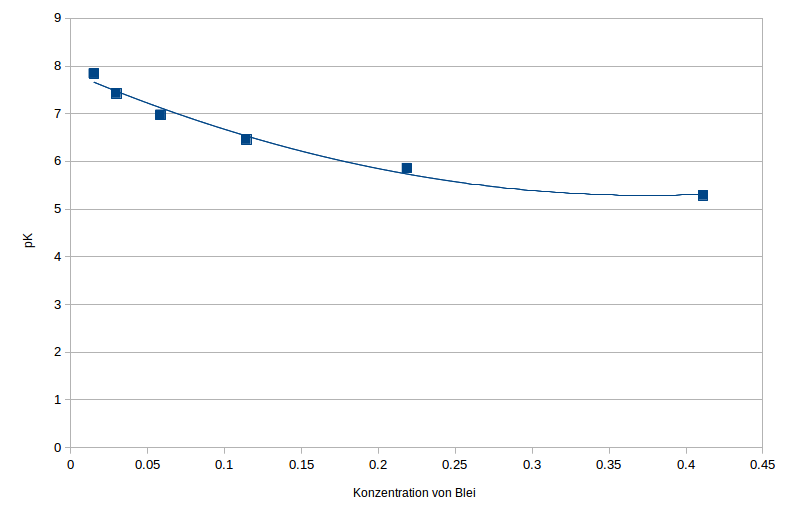
\includegraphics[scale=0.6, center]{Graphiken/Auswertung/Extrapolation.png} 
      \caption[Extrapolationskurve zur Bestimmung von $pK_{L}$ mit LibreOfficeCalc, Quelle: Autor]{LibreOfficeCalc - Extrapolationskurve zur Bestimmung von $pK_{L}$: (x-Achse) $[\ch{Pb\pch[2]\aq}]_{eq.}$ in M, (y-Achse) $pK_{L,c}$; $y=18.281x^2-13.725x+7.862,R^2=0.983$}
      \label{fig:Extrapolation}
    \end{figure}
    
    \begin{figure}[H]
      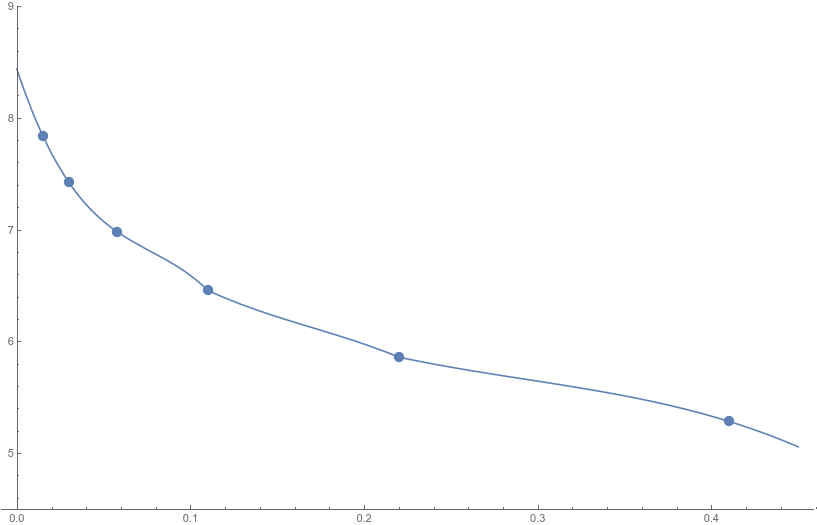
\includegraphics[scale=0.4, center]{Graphiken/Auswertung/ExtrapolationMathematica.png} 
      \caption[Extrapolationskurve zur Bestimmung von $pK_{L}$ mit Mathematica, Quelle: Autor]{Mathematica - Extrapolationskurve zur Bestimmung von $pK_{L}$: (x-Achse) $[\ch{Pb\pch[2]\aq}]_{eq.}$ in M, (y-Achse) $pK_{L,c}$}
      \label{fig:Extrapolationzwei}
    \end{figure}
    
  \pagebreak
  
  \listofreactions
  \printbibliography[title=Literaturverzeichnis]
  \listoffigures
  \listoftables
  
\end{document}
